\section{Generating the task graph}
\label{sec:gener-task-graph}

The compilation tool-chain is described in Figure~\ref{fig:5a}. Our
framework can be used in conjunction with the polyhedral model and other
compiler frameworks described in~\cite{atiw09,ubon08}.  Our framework
takes as input the output from these tuning frameworks, built for single
processing element systems and expands it to a multi-core heterogeneous
architecture.

\begin{figure*}[t!]
  \centering
  \subfigure[The compilation tool-chain]{
    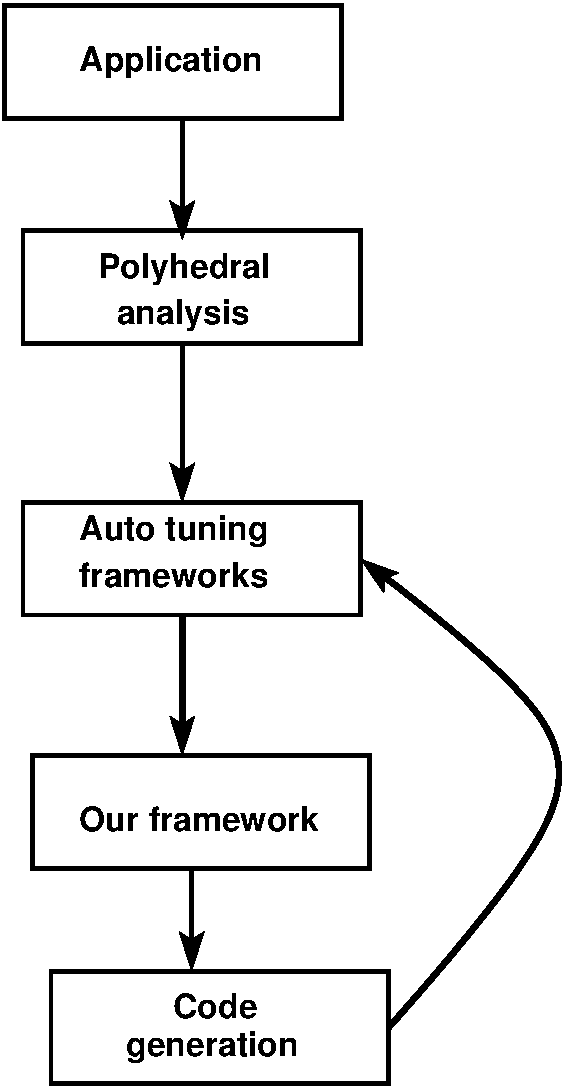
\includegraphics[scale=0.3]{./figures/tool_chain}
    \label{fig:5a}
  }
  \subfigure[The task graph for the Jacobi example]{
    \scalebox{0.4}{\input{./figures/jacobi.pdf_t}}
    % 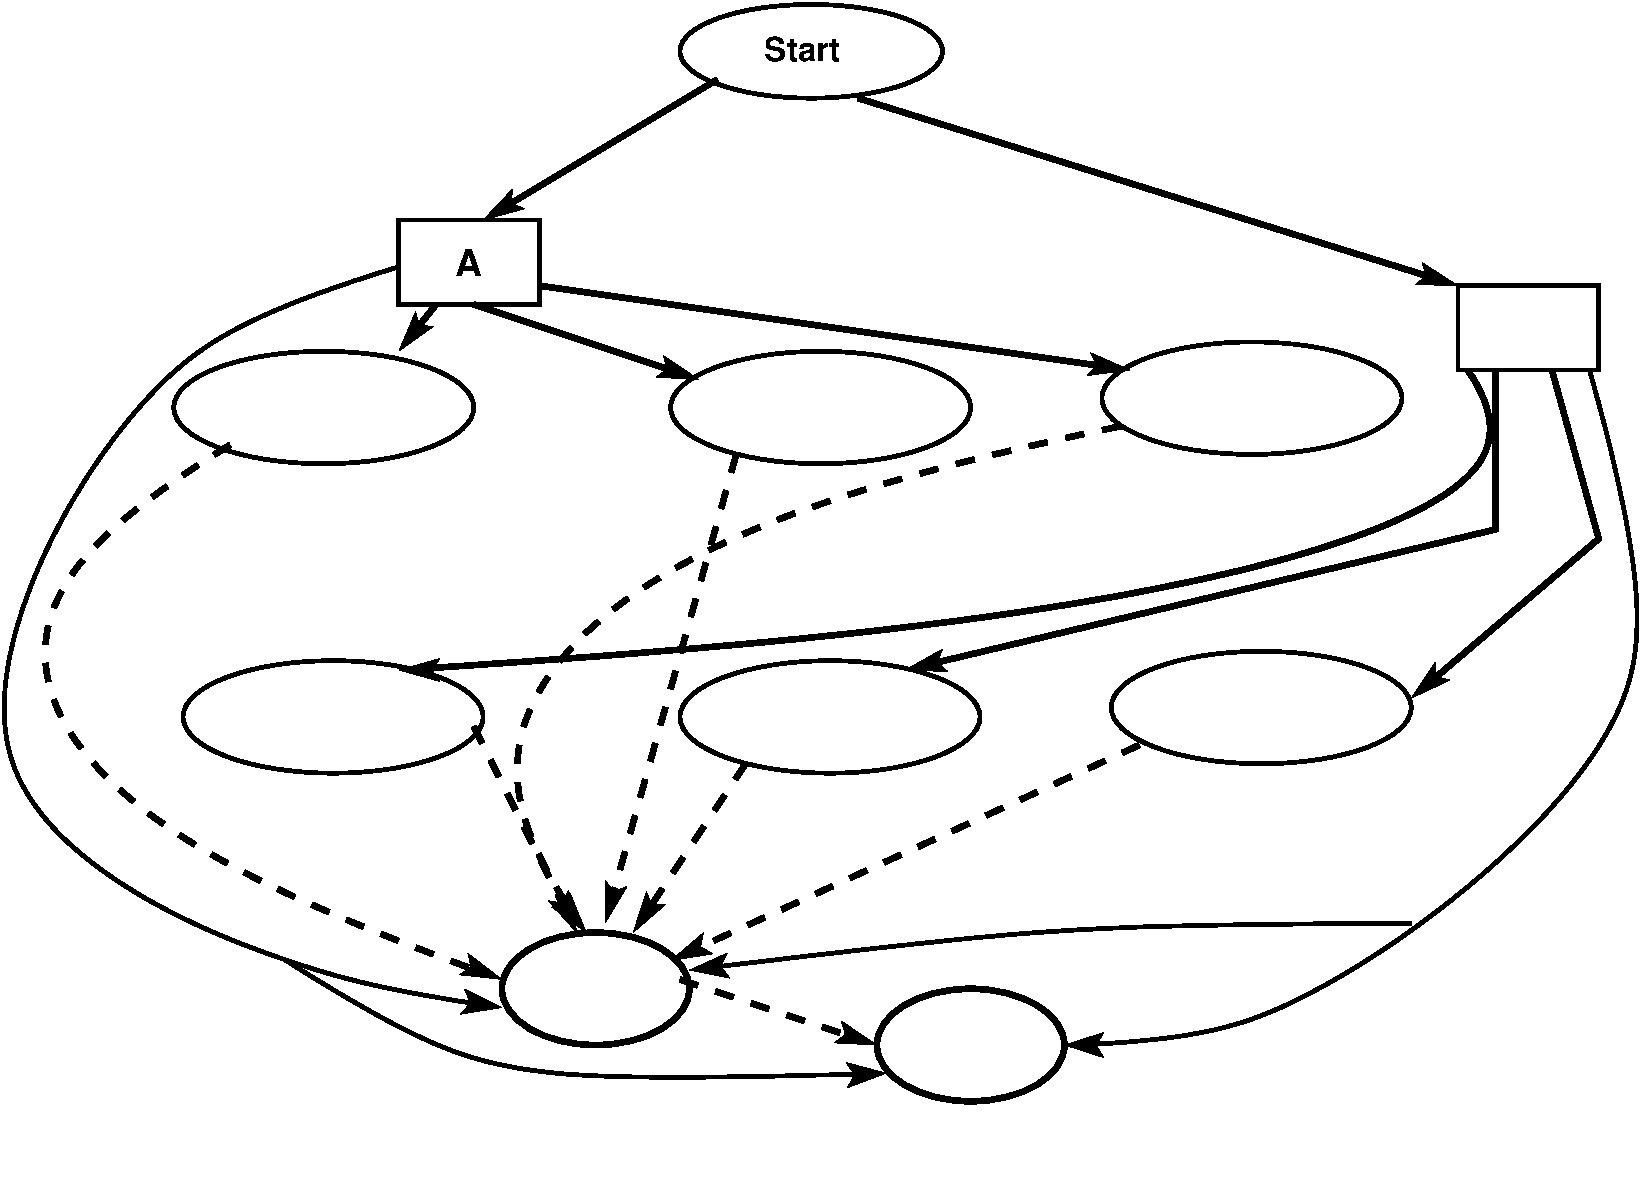
\includegraphics[scale=0.4]{./figures/jacobi}
    \label{fig:5b}
  }
  \caption{Compilation tool-chain and an example task graph}
  \label{fig:5}
\end{figure*}

In this section we use the very popular Jacobi~\cite{jacobi2} stencil
computation to describe how our framework extracts a task graph from the
application for partitioning onto the underlying architecture. Jacobi is
an important stencil computation used in a plethora of domains such as
fluid dynamic and hence, it is worth investigating performance
improvements for Jacobi.

In Figure~\ref{fig:4}, statements S1 and S2 initialize 2D Jacobi
matrices. Next, the actual stencil computation is carried out in
statement S3, for \texttt{TSTEPS} iterations. Finally, statement S4,
transfers the calculated data from matrix \texttt{B} to \texttt{A}.

\begin{scriptsize}
  \begin{figure}[h!]
    \centering
    \small{
\begin{verbatim}
 //Task and data-parallel
 for (int i=0;i<M; ++i){
  for (int j=0;j<N; ++j){
   S1: A[i][j] = (i*j+4.0/N)
   S2: B[i][j] = (i*j+9.0/N)
  }
 }
 for (int k=0;k<TSTEPS;++k){
  for (int i=1; i<M-1; ++i)
   for (int j=1; j<N-1; ++j)
    S3: B[i][j] = 0.2*(A[i][j]+A[i][j-1]
              +A[i][j+1]+A[i-1][j])

  //Data-parallel
  for (int i=1; i<M; ++i)
   for (int j=1; j<N; ++j)
    S4: A[i][j] = B[i][j]
 }
\end{verbatim}
    }
    \caption{Example 2-dimensional Jacobi stencil computation}
    \label{fig:4}
  \end{figure}
\end{scriptsize}

The task graph for the 2D Jacobi stencil computation is shown in
Figure~\ref{fig:5b}. The initialization phase of the Jacobi example
consist of both task and data parallelism. In Figure~\ref{fig:5b}, the
first and second row of statements $S1_1$ to $S1_m$ and $S2_1$ to
$S2_m$, show various loop tiles that are generated for execution onto
different processors for statements S1 and S2, respectively. Each of
these nodes indicate vector computations. Sample vector code within any
one of these assignment nodes when assigned to an Intel SSE3 unit is
shown in Figure~\ref{fig:6}. Similar vector code is generated in the ptx
format for GPU allocations. We keep a count of the number of
instructions for each of these nodes. There are two counts: (1) the
number of instructions a node needs to execute iteratively. For example,
node S3 (representing statement S3 in the Jacobi example) needs to
iterate 998001000 times for a 1000 $\times$ 1000 matrix with
\texttt{TSTEPS} itself set to a 1000, provided it is not vectorized as
shown in Figure~\ref{fig:5b}. (2) Nodes $S1_1$ to $S1_m$ and $S2_1$ to
$S2_m$ only need to be executed once, but have a large vector count.

Each ellipse in the task-graph is connected to a store. Stores are
represented as boxes in the task-graph. Stores have their instruction
count and vector length count set to 0. Every statement depending upon
its vector length requires different amount of data to carry out the
computation. This data needs to be transfered from the store (the main
memory in most cases) to the caches where the task nodes are going to be
executed. We represent the amount of data to be transfered in the
task-graph in bits. For example, node $S1_1$ with a smaller vector
length of 16, requires 2.2KB of data to be transfered to its cache for
computation. Node S3 on the other hand, being non-vectorized requires
15KB of data to be transfered to its cache.

Finally, the task graph also consists of dependence edges. In
Figure~\ref{fig:5b}, the dependence edges are marked with the dashed
lines. Dependence edges, as the name suggests show the dependence
between statements in the application. For example, statements S1 and S2
are independent of each other. But, statements S3 and S4 are dependent
upon these aforementioned statements. Dependence edges do not have any
weights. Once partitioned, the task-graph can then be scheduled
statically or dynamically (work stealing~\cite{rblu99}, say) using these
dependence edges.

\begin{figure}[h!]
  \centering
  \small{
\begin{verbatim}
LCPI0_0:
 .long	1018444121 ## float 2.200000e-02
 .long	1021128475 ## float 2.700000e-02
 .long	1023611503 ## float 3.200000e-02
 .long	1024953680 ## float 3.700000e-02

 movaps	LCPI0_0(%rip), %xmm8
\end{verbatim}
  }
  \caption{Example vector code running on the Intel SSE unit}
  \label{fig:6}
\end{figure}




%%% Local Variables: 
%%% mode: latex
%%% TeX-master: "bare_conf"
%%% End: 
